% Results of the conditioned model with hierarchical tags, H = 128.
% Numbers from evaluations/fa_conditional_H128/{metrics,tree_comparison,mode_mixing}.json

\section{Results: the conditioned model with $H=128$}\label{sec:res_cond}

\subsection{What was trained}
The conditioned model of \S\ref{sec:cond} (hierarchical tags, shared attention, label-specific $\Delta h$ and
$\Delta V$, hierarchical tag dropout 0.10/0.10/0.15) was trained on the same 144{,}000 sequences, with
$\bm{H=128}$ heads like the unconditioned run, so that the two differ only by the conditioning
(run \texttt{fa\_conditional\_H128}, 2{,}115{,}920 parameters, of which 1{,}572{,}000 in the label tables).
Regularisation: $\lambda_h=\lambda_J=10^{-5}$, $\lambda_{\text{label}}=10^{-4}$. Training took 23 minutes and
stopped early at epoch 47. The best epoch is 38.

\begin{figure}[H]
\centering
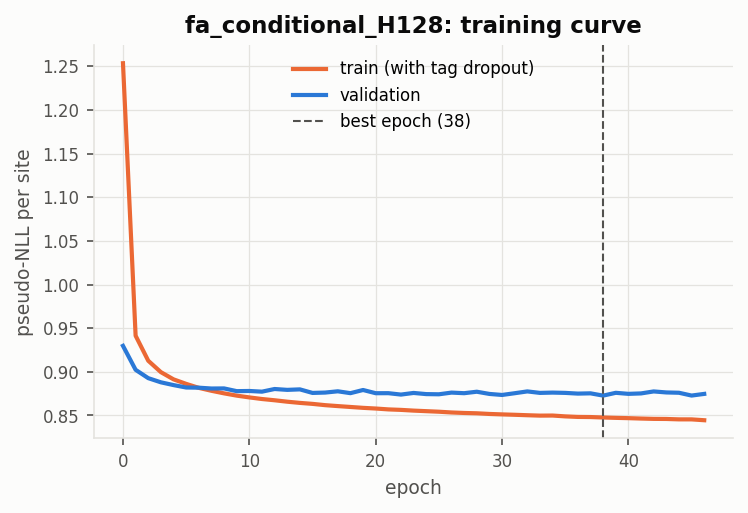
\includegraphics[width=0.55\linewidth]{models/fa_conditional_H128/training_curve.png}
\caption{Training curve. The validation pseudo-NLL (true tags) reaches $0.878$ by epoch 10 and only $0.873$
at the best epoch (38). Meanwhile the training loss keeps decreasing (with tag dropout, so it is not directly
comparable). The label tables start to fit noise beyond epoch $\approx10$.}
\end{figure}

\begin{center}\small
\begin{tabular}{lc}
\toprule
model & validation pseudo-NLL per site\\
\midrule
independent sites, one profile per clade & 1.63\\
unconditioned model ($H=128$) & 0.949\\
\textbf{conditioned model ($H=128$), true tags} & \textbf{0.873}\\
true clade Potts models (floor) & 0.80\\
\bottomrule
\end{tabular}
\end{center}
The tags close about half of the gap between the unconditioned model and the floor.

\subsection{Sequences generated with a clade tag}
For each clade, 1000 sequences were generated with its full tag and compared with that clade's 1000 test
sequences. The oracle is 1000 fresh samples of the true clade model, i.e.\ the noise floor of
\S\ref{sec:refvalues}.
\begin{center}\small
\begin{tabular}{lccccc}
\toprule
mean [min, max] over 18 clades & $r_f$ & $r_C$ & slope $C$ & identity gen / test & copies\\
\midrule
oracle & 0.998 & 0.832 [0.80, 0.88] & 0.84 & 0.337 / 0.337 & 0\%\\
\textbf{generated (clade tag)} & \textbf{0.967} & \textbf{0.758} [0.71, 0.82] & \textbf{0.75} & 0.362 / 0.337 & 0\%\\
\bottomrule
\end{tabular}
\end{center}
On the reference ladder of \S\ref{sec:refvalues} (0.83 same clade, 0.63 sibling clade, 0.35 same family,
0.08 other family), the generated clades score \textbf{0.76}. That is well above the sibling-clade level, so
the generated sequences are closer to their own clade than the true sibling clade is, but still below the
oracle. The generated sequences are slightly too similar to each other (identity 0.36 vs 0.34), and their
correlations are somewhat too weak (slope 0.75 vs 0.84 for the oracle; the oracle slope is below 1 only
because of finite-sample noise).

\begin{figure}[H]
\centering
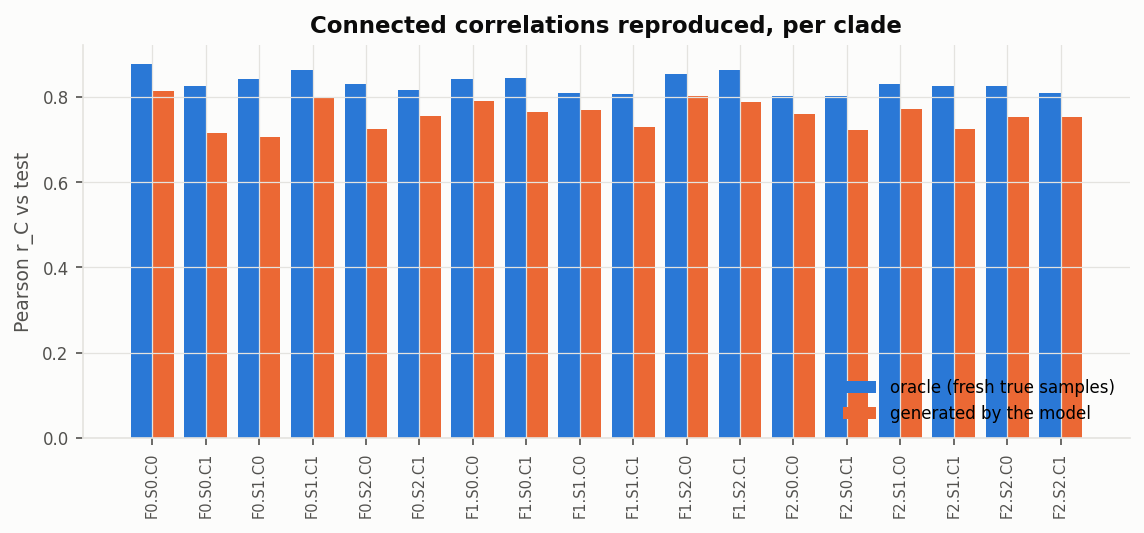
\includegraphics[width=0.8\linewidth]{models/fa_conditional_H128/rC_per_clade.png}
\caption{$r_C$ of each clade's generated sequences vs its test sequences (orange), next to the oracle (blue).
The gap is 0.04--0.14 depending on the clade.}
\end{figure}

\begin{figure}[H]
\centering
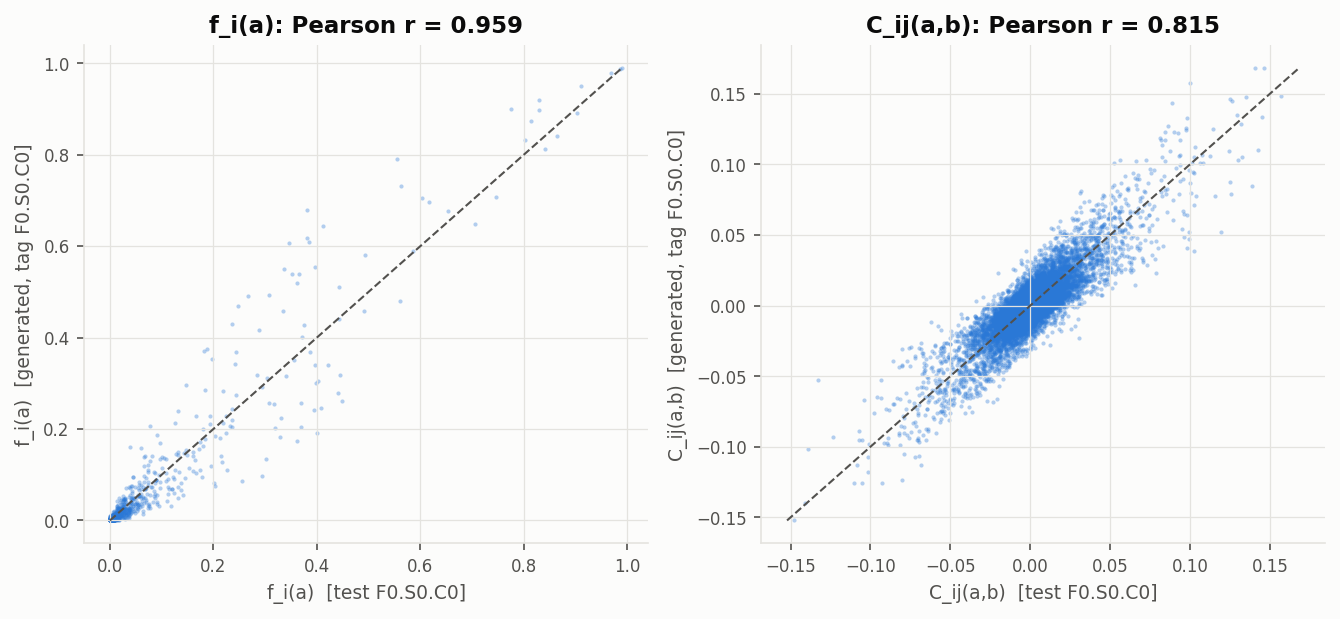
\includegraphics[width=0.49\linewidth]{models/fa_conditional_H128/freq_corr_F0.S0.C0.png}\hfill
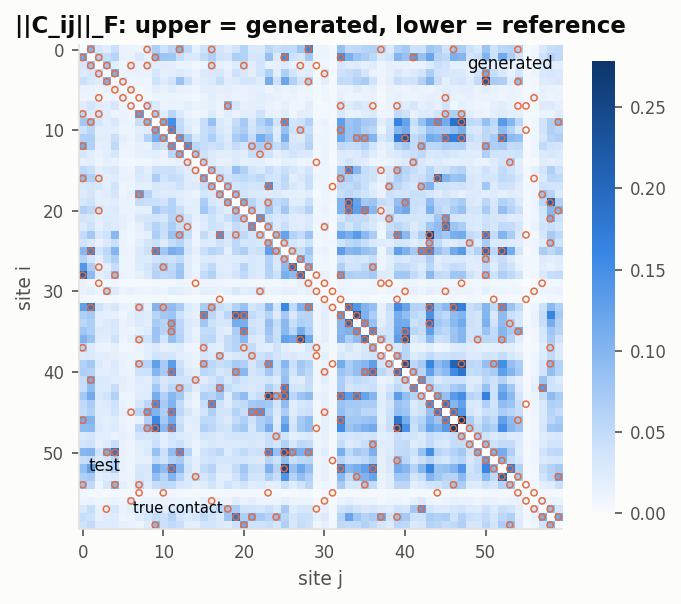
\includegraphics[width=0.4\linewidth]{models/fa_conditional_H128/correlation_strength_F0.S0.C0.png}
\caption{Example clade \texttt{F0.S0.C0}. Left: site frequencies and connected correlations, generated vs
test. Right: correlation strength $\|C_{ij}\|$, test (lower triangle) vs generated (upper), true contacts
circled. Within one clade the strongest correlations sit on true contacts. The weaker background comes from
indirect correlations and finite-sample noise (1000 sequences).}
\end{figure}

\begin{figure}[H]
\centering
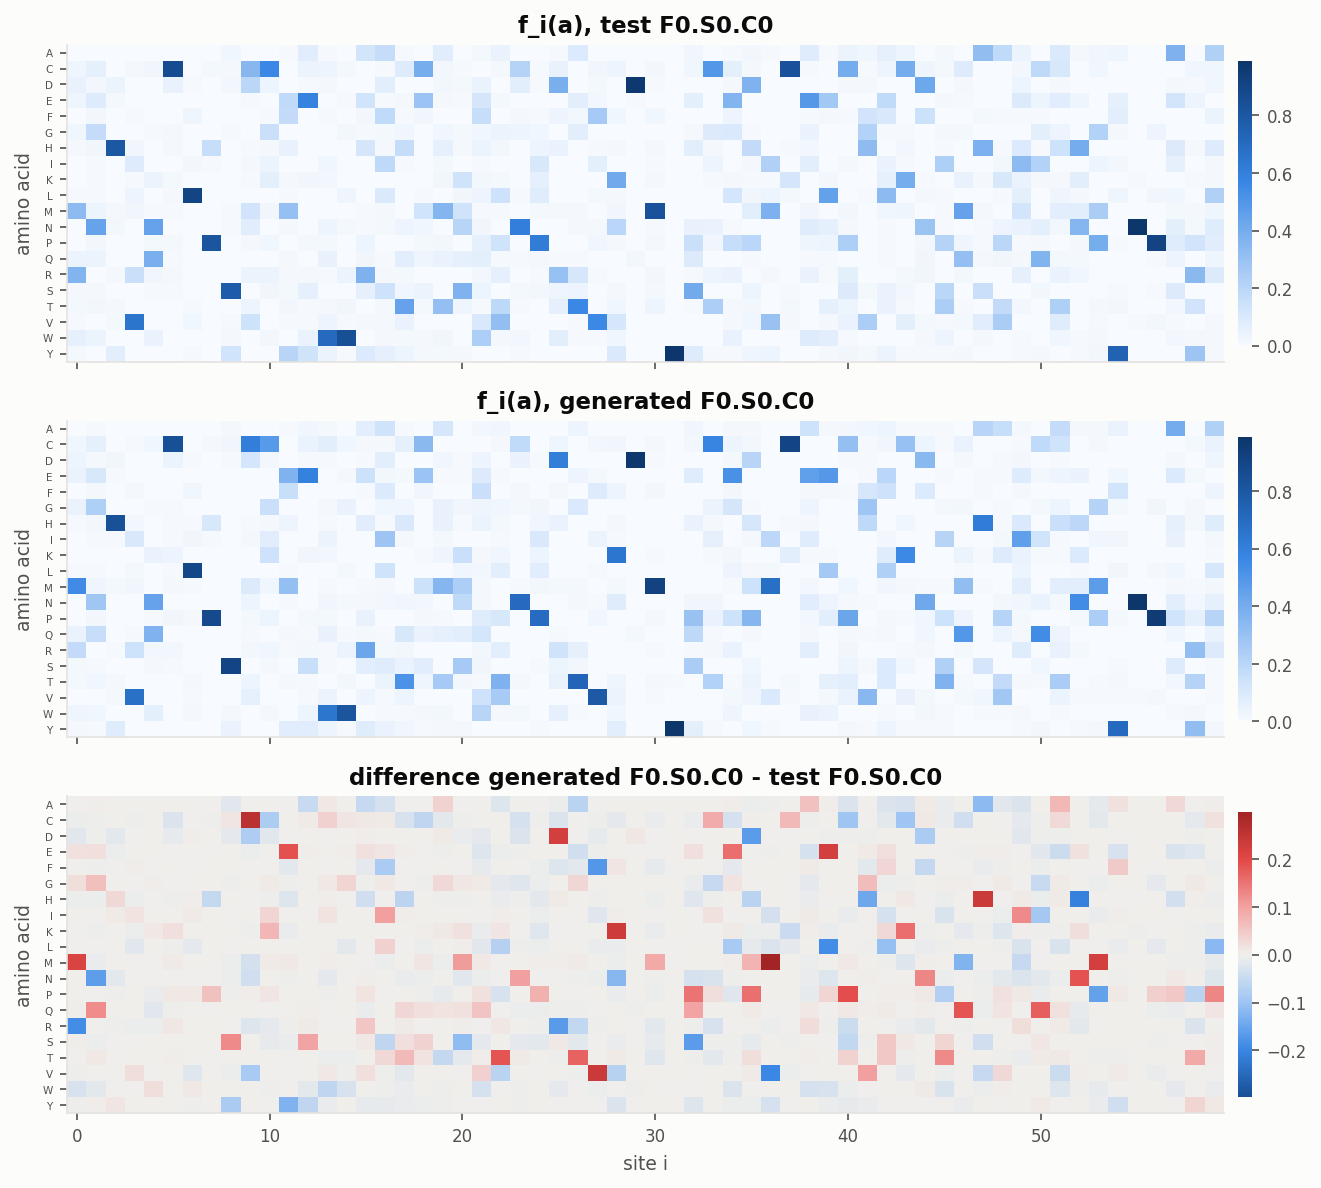
\includegraphics[width=0.78\linewidth]{models/fa_conditional_H128/site_frequencies_F0.S0.C0.png}
\caption{Site frequencies of clade \texttt{F0.S0.C0}: test, generated with its tag, and the difference.}
\end{figure}

\paragraph{Does the tag select the right clade?} For every pair (generated clade $a$, test clade $b$) we
compute $r_C$. \textbf{All 18 generated clades are closest to their own test clade} (assignment accuracy
100\%), and the matrix reproduces the hierarchy of the data: sibling clades next, then the same family.
\begin{figure}[H]
\centering
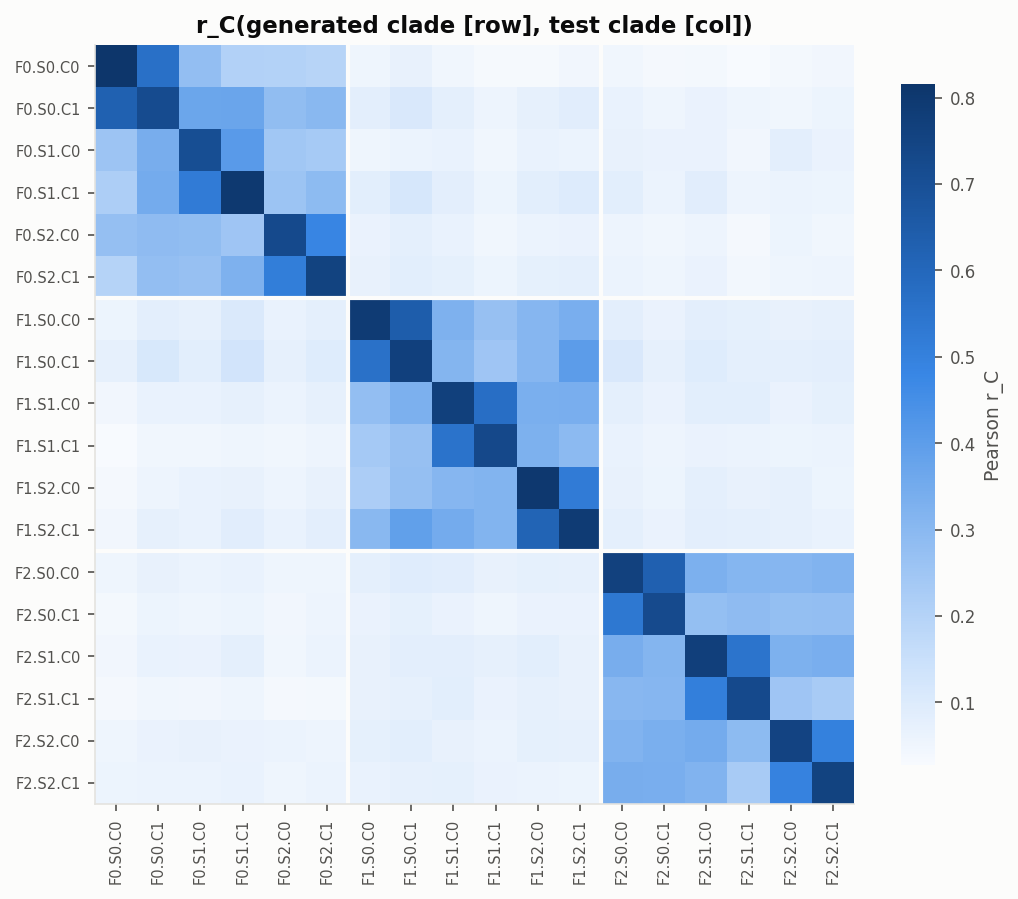
\includegraphics[width=0.62\linewidth]{models/fa_conditional_H128/cross_clade_rC.png}
\caption{$r_C$ between generated clade (row) and test clade (column). The diagonal dominates every row, and
the block structure (pairs of sibling clades, then families) is that of the ground truth.}
\end{figure}

\begin{figure}[H]
\centering
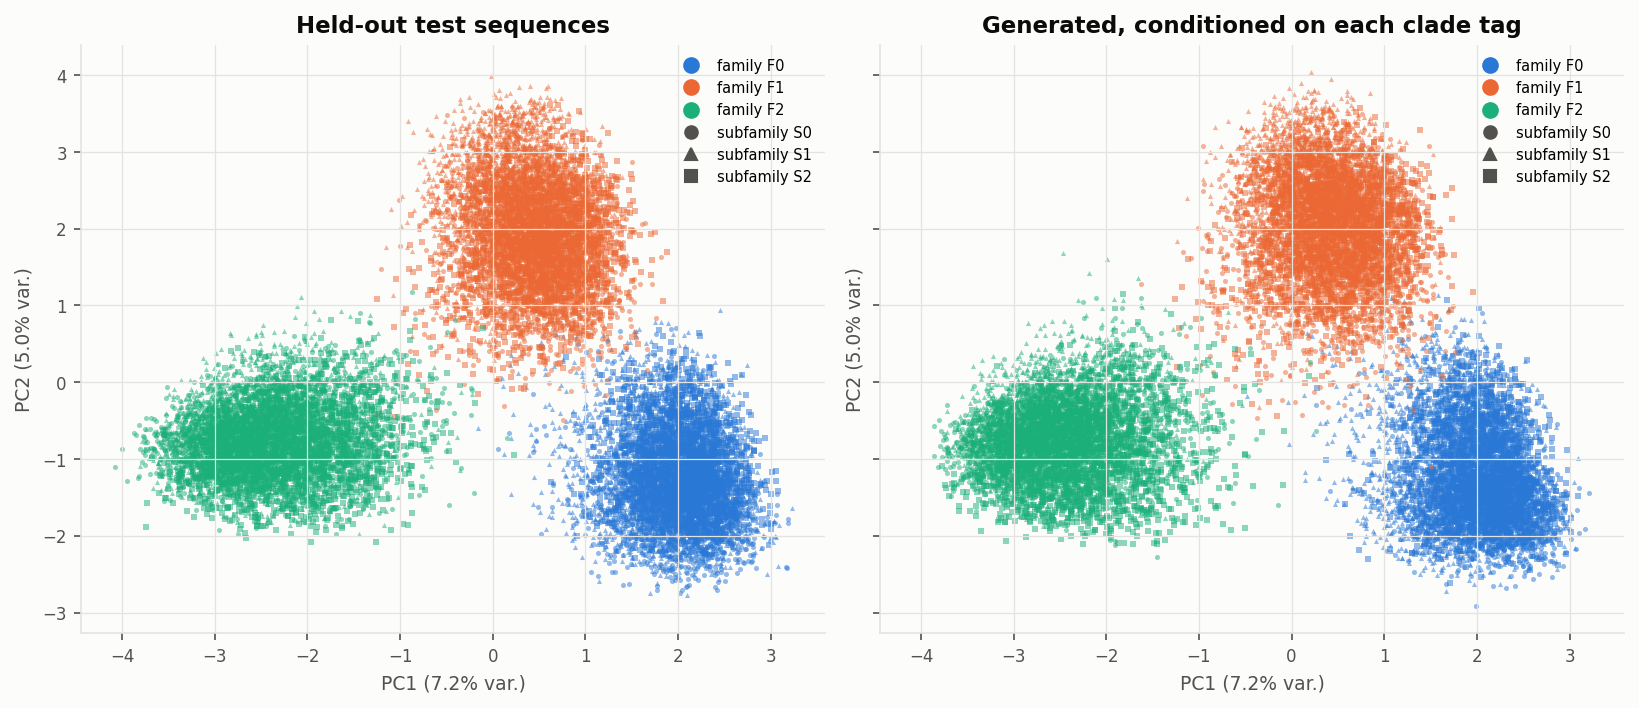
\includegraphics[width=0.85\linewidth]{models/fa_conditional_H128/pca_generated_vs_test.png}
\caption{Test sequences (left) and sequences generated with each of the 18 clade tags (right) on the reference
PCA. Pooled over the 18 tags, the generated set has exactly the right family shares (32.8/32.9/33.3\%) and
$r_f=0.992$, $r_C=0.954$ against the whole test set.}
\end{figure}

\subsection{Sequences generated with a family tag, or with no tag}
\begin{center}\small
\begin{tabular}{lccccc}
\toprule
tag & $r_f$ & $r_C$ & slope $C$ & \multicolumn{2}{c}{family of the generated sequences}\\
\midrule
family F0 only & 0.986 & 0.841 & 0.71 & \multicolumn{2}{c}{99.4\% in F0}\\
family F1 only & 0.984 & 0.856 & 0.73 & \multicolumn{2}{c}{97.8\% in F1}\\
family F2 only & 0.990 & 0.850 & 0.67 & \multicolumn{2}{c}{99.4\% in F2}\\
no tag & 0.980 & 0.872 & 0.52 & \multicolumn{2}{c}{F0/F1/F2 $=$ 33/21/46\%}\\
\bottomrule
\end{tabular}
\end{center}
(Family-tag samples are compared with the whole family's test set, 6000 sequences; no-tag samples with the
whole test set.)
\begin{itemize}
\item \textbf{A family tag generates that family}, 98--99\% of the time, with good statistics. This is
      what the unconditioned model could not do.
\item \textbf{With no tag the family weights are still wrong} (33/21/46\%), although less so than for the
      unconditioned model (22/12/66\%). This is the same pseudo-likelihood blind spot as in
      \S\ref{sec:res_props}. The no-tag mode is fitted to the whole mixture (10\% of training sequences have no
      tag). The energy/entropy breakdown (\texttt{s08}) shows the same near-cancellation as before: relative to F2, F0
      has an energy term $-9.4$ and an entropy term $+9.2$ (net $-0.27$), and F1 has $-14.1$ and $+13.3$ (net
      $-0.77$). With tags, the family weights are \emph{chosen by the user}, so this blind spot no longer matters for
      generation: pooling equal numbers of clade-tag samples gives exactly 1/3 per family (previous figure).
\end{itemize}

\subsection{The learned $J(\text{tag})$ compared with the right tensors}
Each tree node has a tag that should reproduce it: the root $\leftarrow$ no tag; family F$f$ $\leftarrow$
tag $(f,-,-)$; subfamily $\leftarrow$ family $+$ subfamily tag; clade $\leftarrow$ full tag. So we have 31
learned models for 31 true ones. Each learned $J(\text{tag})$ was compared with every true $J$
(\texttt{s07\_compare\_to\_tree.py}); the \emph{matched} comparison is the diagonal.

\begin{figure}[H]
\centering
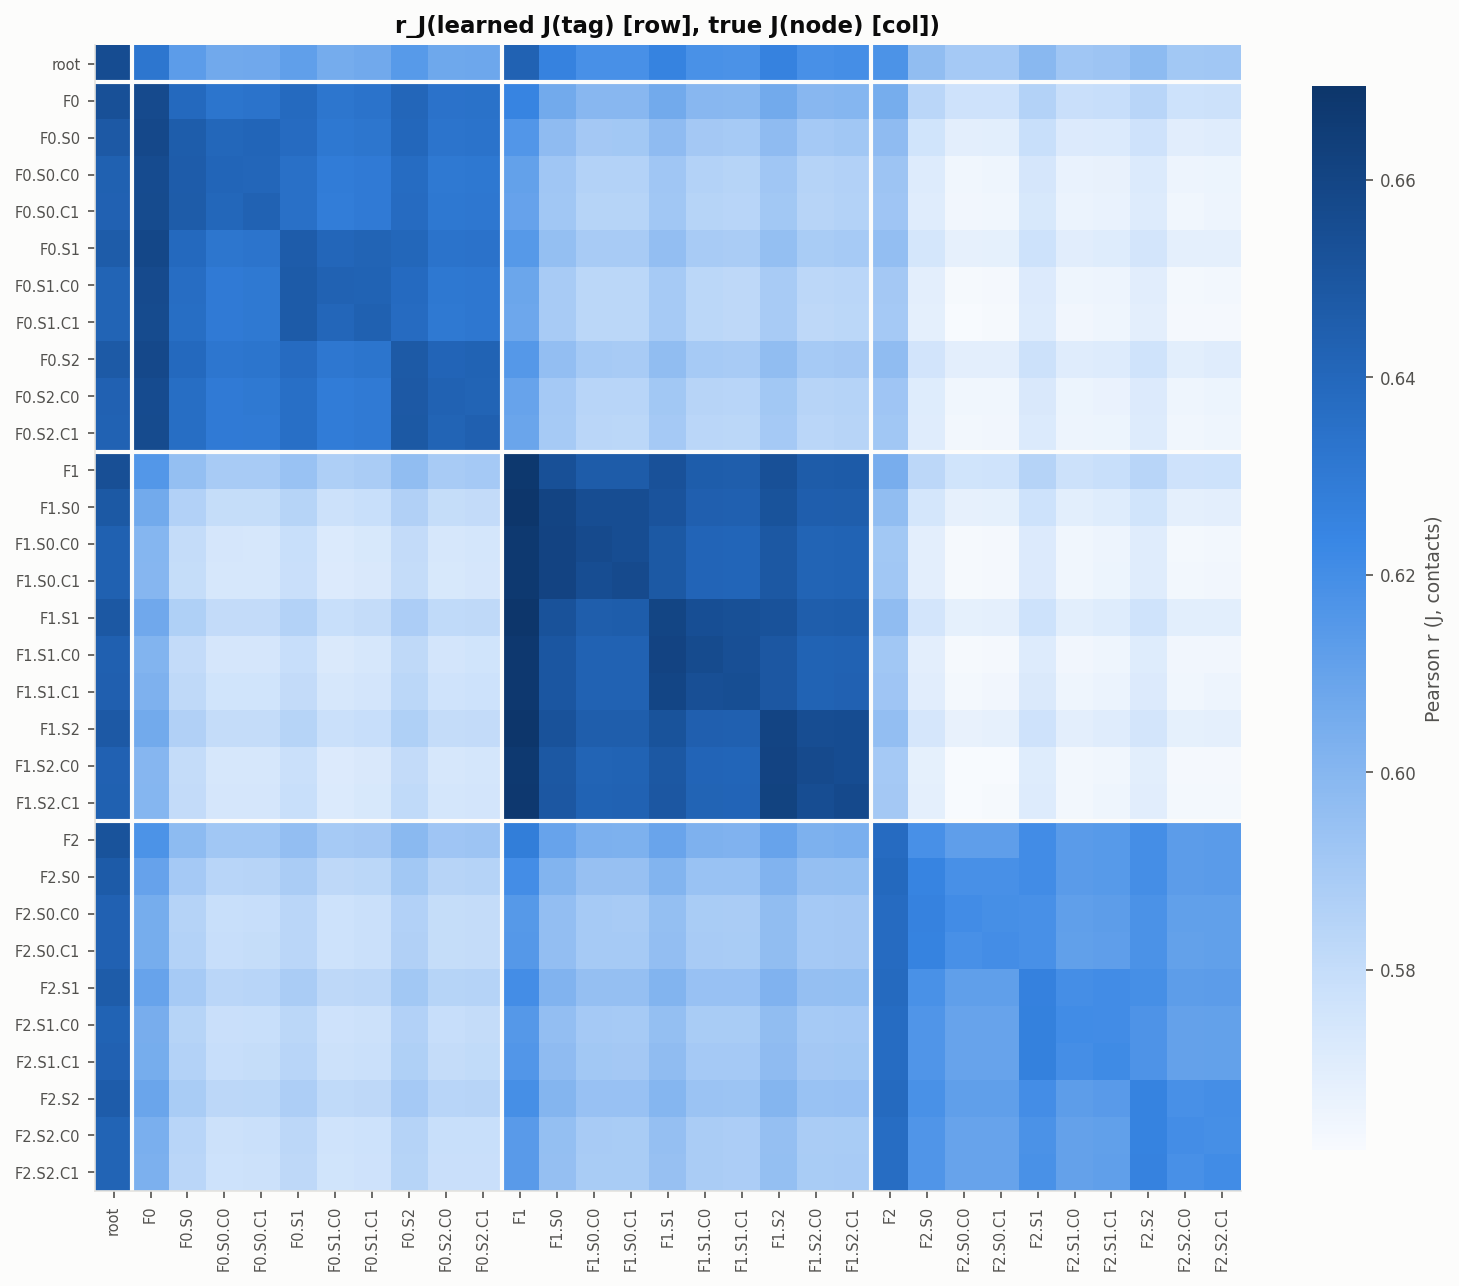
\includegraphics[width=0.8\linewidth]{models/fa_conditional_H128/tree_matrix_rJ.png}
\caption{Pearson $r_J$ (contact entries, zero-sum gauge) between the learned $J$ of each tag (rows) and every
true $J$ (columns). A perfect model would have a dark diagonal. What we see is a clear \emph{family} block
structure: every tag's $J$ resembles its own family (and the root) more than any other family. Within a
family block, however, the rows differ only slightly (a faint subfamily diagonal): the couplings barely
distinguish subfamilies and clades.}
\label{fig:matrixJ}
\end{figure}

\begin{center}\small
\begin{tabular}{lcccccc}
\toprule
level of the tag & $n$ & matched $r_J$ & matched slope & matched $r_h$ & $r(\Delta J)$ & $r(\Delta h)$\\
\midrule
none (root) & 1 & 0.655 & 0.46 & 0.871 & -- & --\\
family & 3 & 0.654 & 0.42 & 0.889 & 0.34 & 0.58\\
subfamily & 9 & 0.644 & 0.41 & 0.882 & 0.21 & 0.50\\
clade & 18 & 0.640 & 0.40 & 0.871 & 0.11 & 0.33\\
\bottomrule
\end{tabular}
\end{center}
Here $r(\Delta J)$ is the correlation between the learned change of couplings from the parent tag to the child
tag, $J(\text{child tag})-J(\text{parent tag})$, and the \emph{true} change $J_{\text{child}}-J_{\text{parent}}$
(contact entries, zero-sum gauge); $r(\Delta h)$ is the same for the fields. They measure whether the model
learned what is \emph{specific} to a label, rather than what it shares with its parent.

\begin{figure}[H]
\centering
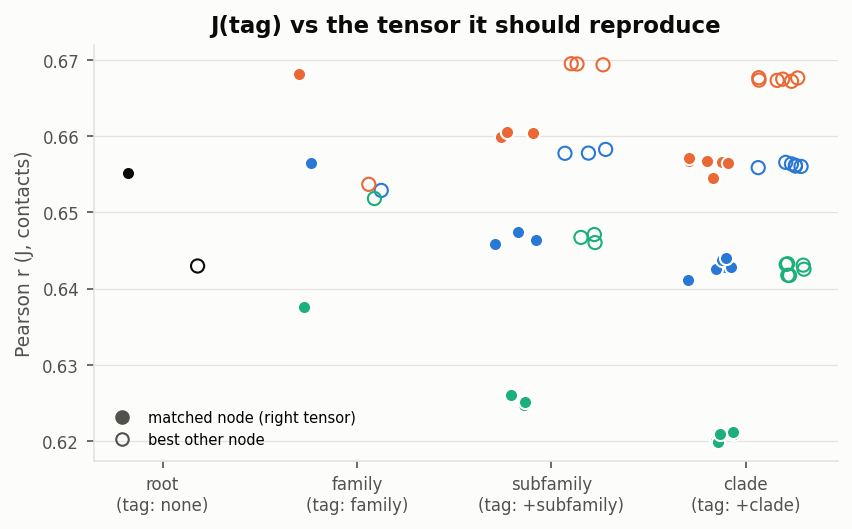
\includegraphics[width=0.55\linewidth]{models/fa_conditional_H128/tree_matched_rJ.png}
\caption{For each tag: $r_J$ with the tensor it should reproduce (filled) and with the best \emph{other} tensor
(open). At the family level the matched tensor wins for F0 and F1. At the subfamily and clade levels, another
tensor (always the tag's own family, or the root) correlates slightly better than the matched one.}
\end{figure}

By $r_J$, the true tensor that best matches each tag's $J$ is:
\begin{center}\small
\begin{tabular}{lcccc}
\toprule
level of the tag & itself & its own family & the root & another family\\
\midrule
family (3) & 2 & -- & 1 & 0\\
subfamily (9) & 0 & 6 & 3 & 0\\
clade (18) & 0 & 12 & 6 & 0\\
\bottomrule
\end{tabular}
\end{center}

\paragraph{Reading.}
\begin{enumerate}
\item \textbf{The couplings resolve the family, not the subfamily or the clade.} No tag's $J$ ever best
matches another family, but below the family level $J(\text{tag})$ is essentially the family's $J$. The
label-specific part of the couplings is weak and gets weaker with depth: $r(\Delta J)=0.34\to0.21\to0.11$.
\item \textbf{The fields carry the finer labels.} $r(\Delta h)=0.58\to0.50\to0.33$, about twice
$r(\Delta J)$ at every level. This is how the clade tags still select the right clade (100\% assignment
accuracy): the clade-specific conservation is learned in $h$.
\item \textbf{Why are the label-specific couplings weak?} Two reasons, both predictable from the architecture.
  (i) \emph{Capacity}: the label changes $J$ only through $\sum_hA^h_{ij}\Delta V^h(\text{tag})$, with the
  \emph{shared} attention and $H=128$ value matrices. The true clade perturbations are independent random blocks
  on 179 contacts, so by the rank argument of \S\ref{sec:rank} at most 128 of the 179 independent directions
  can be represented. (ii) \emph{Signal}: the true clade perturbations are small ($\sigma_J^{(3)}=0.15$, against
  0.8 for the root). Each clade tag sees only 8000 sequences, and the label tables are penalised
  ($\lambda_{\text{label}}$). The flat validation curve after epoch 10 shows that the extra label parameters
  mostly fit noise beyond that point.
\item \textbf{All couplings are shrunk.} The matched slope is $0.40$--$0.46$, i.e.\ the couplings along the
true direction are less than half their true size (0.57 in the unconditioned model). Part of the correlation
structure is instead carried by sharper fields: the generated sequences are slightly too conserved (identity
0.36 vs 0.34). Contact precision is still 1.00 for every tag.
\end{enumerate}

\subsection{Unconditioned vs conditioned}
\begin{center}\small
\begin{tabular}{p{0.36\linewidth}p{0.2\linewidth}p{0.34\linewidth}}
\toprule
 & unconditioned & conditioned (tags)\\
\midrule
validation pseudo-NLL per site & 0.949 & 0.873\\
family shares of generated sequences & 22/12/66\% & chosen by the tag (33/33/33\% pooled; 98--99\% correct per family tag)\\
$r_C$ per clade (oracle 0.83) & -- (no clade control) & 0.76\\
$r_C$ pooled (oracle 0.994) & 0.895 & 0.954\\
generated clade closest to its own test clade & -- & 18/18\\
$J$ resolves & the ancestor (root) & the family\\
long-range contact precision & 1.00 & 1.00\\
\bottomrule
\end{tabular}
\end{center}

\begin{keybox}{Conditioned model with $H=128$}
\begin{itemize}[nosep]
\item[+] Tags work: a clade tag generates its clade (18/18), a family tag its family (98--99\%), and pooling
      the tags gives the right family proportions. This removes the main failure of the unconditioned model.
\item[+] Per clade, $r_C=0.76$: between the sibling-clade level (0.63) and the noise floor (0.83).
\item[--] The learned couplings resolve only the family; subfamily and clade differences are carried mainly by
      the fields. All couplings are shrunk to $\approx40\%$ of their true size, and correlations are 10\% too weak.
\item[--] Without a tag the family weights are still off (33/21/46\%): the same pseudo-likelihood blind spot.
\end{itemize}
Levers to try next: $H=256$ (removes the rank bound on the label-specific couplings), label-specific
attention (lets tags change \emph{where} the couplings sit, not only their values), a smaller
$\lambda_{\text{label}}$ or more sequences per clade.
\end{keybox}
